% 本文件是第三章机械臂设计小节中的第三小节,主要讲机械臂设计过程中轴的计算。
% 作者:谭正
% 上次更新:2020年1月14日09点57分

\subsection{轴的设计和验算}

\subsubsection{轴的结构设计}

\begin{enumerate}
    \item   蜗杆的结构设计为一端装轴承,一端直接和电机的轴用键连接,如图~\ref{fig:wormsd1}所示。
        \begin{figure}
            \centering
            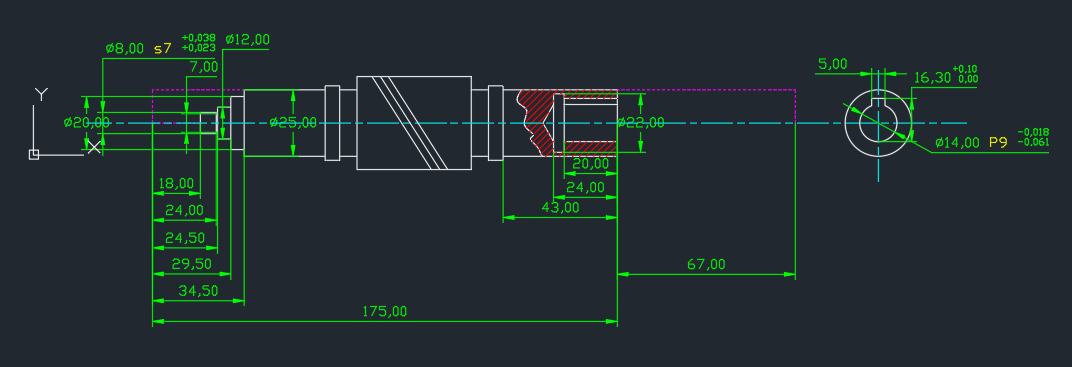
\includegraphics[width=0.8\textwidth]{wormshaftd1.png}
            \bicaption[蜗杆的结构设计]{蜗杆的结构设计(以2.5M的为例)}{Structural design drawing of worm (take 2.5M as an example)}
            \label{fig:wormsd1}
        \end{figure}

    \item   云台上的主轴由于所受弯矩最大,所以给加了四个轴承支座作支撑。其结构设计如图~\ref{fig:rpmain}所示。
        \begin{figure}
            \centering
            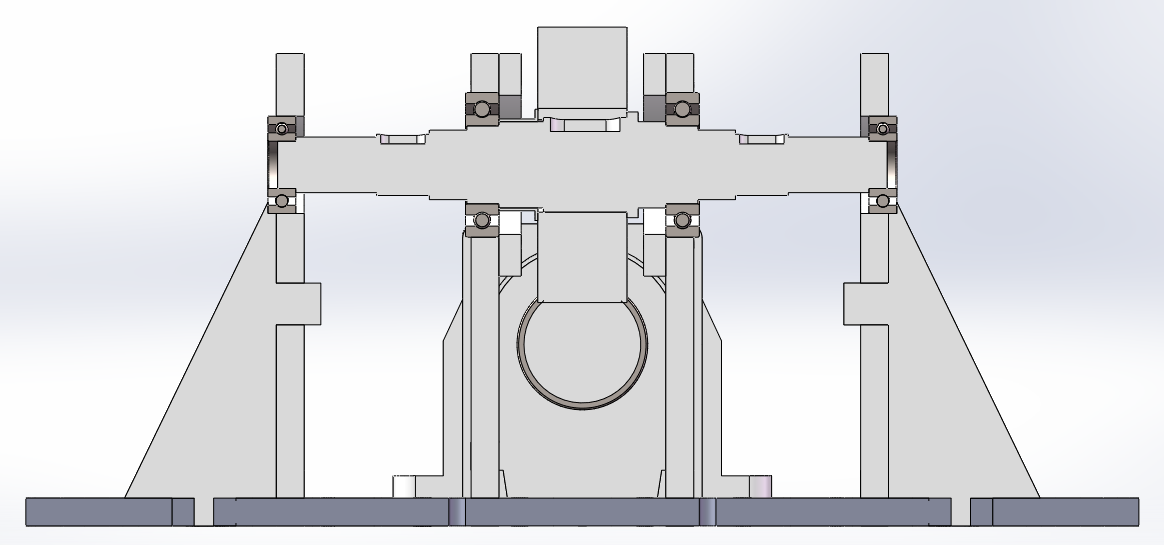
\includegraphics[width=0.8\textwidth]{RPshaft.png}
            \bicaption[云台主轴结构设计]{云台主轴结构设计}{Structural design of gimbal spindle}
            \label{fig:rpmain}
        \end{figure}

    \item   大臂和前臂相连的关节处有布置在悬伸端的同步带轮,为了改善轴的受力情况,使用如图~\ref{fig:arm12s}所示的卸载结构,使转轴变成心轴,只承受弯矩提高了旋转精度。
        \begin{figure}
            \centering
            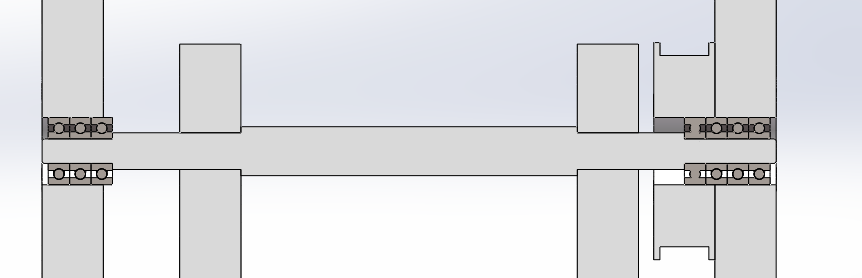
\includegraphics[width=0.8\textwidth]{arm12shaft.png}
            \bicaption[大臂和前臂相连的关节轴的结构设计]{大臂和前臂相连的关节轴的结构设计}{Structural design of the joint shaft connecting the arm 1 and arm 2}
            \label{fig:arm12s}
        \end{figure}

    \item   前臂和腕部相连接的关节处也采用了类似的思想来减小载荷。如图~\ref{fig:arm23s}所示。
        \begin{figure}
            \centering
            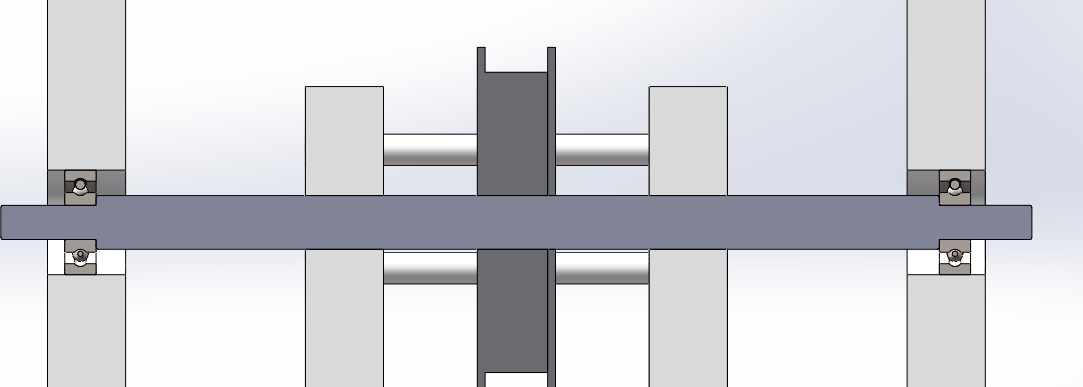
\includegraphics[width=0.8\textwidth]{arm23shaft.png}
            \bicaption[前臂与腕部连接处的轴的结构设计]{前臂与腕部连接处的轴的结构设计}{Structural design of the shaft at the junction of the arm 2 and the arm 3}
            \label{fig:arm23s}
        \end{figure}

    \item   驱动腕部的电机轴同蜗杆,也采用了带键槽的盲孔设计。
\end{enumerate}

\subsubsection{轴的强度、刚度计算}
    在进行强度计算时,对应不同类型的轴有不同的计算方法来估计其最小截面。
    \begin{enumerate}
        \item   对于转轴,同时承受弯矩和转矩,应满足第四强度理论计算公式~\ref{eq:forth}。
            \begin{equation}
                \label{eq:forth}
                \sigma _{ca} = \sqrt{\left( \frac{M}{W}\right)^2 + 4\left(\frac{\alpha T}{W_T}\right)^2}
                \approx 
                \frac{\sqrt{M^2 + (\alpha T)^2}}{W}
                \leq [\sigma _{-1}]
            \end{equation}
        
        \item   对于心轴,只承受弯矩,应满足式~\ref{eq:wanju}
            \begin{equation}
                \label{eq:wanju}
                \sigma _{ca} = \frac{M}{W} \leq [\sigma _{-1}]
            \end{equation}
        \end{enumerate}
        而具体到本装置中所使用的轴,云台主轴所受约束较多,直接用材料力学的方法去计算有些困难,采用有限元分析的方法\footnote{参见下一小节}辅助设计。其余轴都很简单,本小节不再一一细说。
        
        在进行刚度计算时,先进行扭转刚度计算,对于本装置中使用的阶梯轴,需要校核其扭转角,计算公式参见式~\ref{eq:niuzhuan}
        \begin{equation}
            \label{eq:niuzhuan}
            \phi = 5.73\times 10^4 \frac{1}{LG}\sum_{i=i}^{z}\frac{T_i l_i}{I_{Pi}}
        \end{equation}
        在进行弯曲刚度计算时,对于本装置中用到的阶梯轴,均可以用当量直径法\cite{MMDM}作近似计算,校核挠度、偏转角。